% TODO: Bei deskriptiven Grafiken zitieren (Stand 07.03.2025)
% TODO: Durchlesen (Stand 07.03.2025)

\section{Ergebnisse}

%%%%%%%%%%%%%%%%%%%%%%%%%%
% Deskriptive Ergebnisse %
%%%%%%%%%%%%%%%%%%%%%%%%%%

\subsection{Deskriptive Ergebnisse}

% Deskriptive Statistik: Einleitung
Die deskriptiven Statistiken der analysierten Variablen bieten einen umfassenden Einblick 
in deren Eigenschaften und Verteilungen über die beobachteten Länder und Zeiträume. Im 
Folgenden werden die Ergebnisse detailliert beschrieben:

% TODO: - (Stand 04.03.2025)

\begin{table}[H]
\caption{Übersicht über die Variablen}
\resizebox{\textwidth}{!}{
\centering
\begin{tabular}[t]{lrrrrrr}
\toprule
Variable & Min & Max & Mean & Median & SD & N\\
\midrule
UNEMPLOYMENT\_RATE\_PERCENT & 0.82 & 49.89 & 7.95 & 5.96 & 6.34 & 11919\\
ICT\_INVEST\_SHARE\_GDP & 0.73 & 8.69 & 2.46 & 2.25 & 0.98 & 11919\\
GDP\_PER\_CAPITA & 13.34 & 137.72 & 43.73 & 41.27 & 17.13 & 11919\\
PERCENT\_EMPLOYEES\_TUD & 4.50 & 92.20 & 28.45 & 20.40 & 20.71 & 11919\\
PERCENT\_TERTIARY\_EDUCATION & 12.87 & 59.96 & 33.65 & 34.56 & 9.27 & 11919\\
\addlinespace
REGULATION\_STRICTNESS & 0.00 & 4.88 & 2.19 & 2.26 & 0.83 & 11919\\
\bottomrule
\end{tabular}
}
\label{tab:variables_codebook}
\end{table}


% Deskriptive Statistik: Variable "ICT-Investitionen"
Die Variable \textit{\ac{ICT}-Investitionen}, welche den Anteil der Investitionen in 
\ac{ICT} am \ac{BIP} misst \parencite{oecd2022ict}, variiert zwischen einem Minimum von 
0,73\% und einem Maximum von 8,69\%. Der Mittelwert beträgt 2,46\%, während der Median mit 
2,25\% leicht darunter liegt. Dies deutet auf eine leicht rechtsschiefe Verteilung hin, 
da einige Länder besonders hohe Investitionen in \ac{ICT} tätigen. Die Standardabweichung 
von 0,98 zeigt, dass es zwischen den OECD-Ländern erhebliche Unterschiede in der Intensität 
der \ac{ICT}-Investitionen gibt. Während einige Länder konstant hohe Anteile ihrer 
wirtschaftlichen Ressourcen in digitale Technologien investieren, gibt es andere, die 
vergleichsweise geringe Investitionen tätigen. Diese Unterschiede können durch verschiedene 
Faktoren beeinflusst sein, darunter wirtschaftliche Leistungsfähigkeit, politische 
Strategien zur Förderung der Digitalisierung sowie strukturelle Unterschiede in der 
Entwicklung des \ac{ICT}-Sektors.

% Deskriptive Statistik: Variable "Arbeitslosenquote"
Die Variable \textit{Arbeitslosenquote}, welche die Arbeitslosenquote in Prozent angibt 
\parencite{oecd2022unemployment}, schwankt erheblich zwischen einem Minimum von 0,82\% und 
einem Maximum von 49,89\%. Der Mittelwert liegt bei 7,95\%, während der Median mit 5,96\% 
etwas niedriger ausfällt. Dies weist auf eine rechtsschiefe Verteilung hin, da einige 
Länder oder Zeitpunkte mit sehr hohen Arbeitslosenquoten als Ausreißer wirken können. Die 
hohe Standardabweichung von 6,34 deutet darauf hin, dass die Arbeitslosenquoten 
zwischen den Ländern und über die Zeit hinweg erhebliche Unterschiede aufweisen. Während 
einige OECD-Länder durch eine geringe Arbeitslosenquote und stabile Arbeitsmärkte 
gekennzeichnet sind, zeigen andere Länder insbesondere in wirtschaftlichen Krisenzeiten 
oder strukturschwachen Regionen signifikant höhere Arbeitslosenraten. Diese Heterogenität 
könnte zudem mit unterschiedlichen Arbeitsmarktregulierungen und Bildungssystemen 
zusammenhängen.

% Deskriptive Statistik: Variable "BIP pro Kopf"
Das \textit{\ac{BIP} pro Kopf}, welches das Pro-Kopf-Einkommen in Tausend US-Dollar angibt 
\parencite{oecd2022gdp}, weist eine erhebliche Spannweite auf: Es reicht von 13,34 bis 
137,72 Tausend US-Dollar. Der Mittelwert beträgt 43,73 Tausend US-Dollar, während der 
Median mit 41,27 Tausend US-Dollar nur geringfügig darunter liegt. Trotz dieser relativen 
Nähe deutet die hohe Standardabweichung von 17,13 darauf hin, dass es erhebliche 
Wohlstandsunterschiede zwischen den \ac{OECD}-Ländern gibt. Dies spricht für eine starke 
rechtsschiefe Verteilung, da einige besonders wohlhabende Länder den Durchschnittswert 
nach oben treiben.

Diese Unterschiede sind insbesondere für die Interpretation der \ac{ICT}-Investitionen 
relevant, da wohlhabendere Länder tendenziell eine höhere Kapitalausstattung und damit 
größere Investitionsmöglichkeiten in digitale Infrastruktur haben könnten. Gleichzeitig 
können Unterschiede im \ac{BIP} pro Kopf Einfluss auf die Struktur des Arbeitsmarktes und 
damit auf die Verteilung der Arbeitslosigkeit nach Bildungsgrad haben.

% Deskriptive Statistik: Variable "Gewerkschaftsdichte"
Die Variable \textit{Gewerkschaftsdichte}, welche die gewerkschaftliche Organisationsrate 
eines Landes misst \parencite{oecd2022tud}, zeigt eine erhebliche Varianz zwischen den 
Ländern. Die Werte reichen von einem Minimum von 4,50\% bis zu einem Maximum von 92,20\%. 
Der Mittelwert beträgt 28,45\%, während der Median mit 20,40\% darunter liegt, was darauf 
hindeutet, dass einige Länder eine besonders hohe Gewerkschaftsbindung haben, während die 
Mehrheit unter diesem Durchschnittswert bleibt. Die Standardabweichung von 20,71 
verdeutlicht die große Heterogenität in der gewerkschaftlichen Organisation zwischen den 
Ländern. Während einige nordische Länder traditionell hohe Gewerkschaftsdichten aufweisen, 
sind Gewerkschaften in anderen \ac{OECD}-Staaten weniger stark in den Arbeitsmarkt 
integriert. Dies könnte Implikationen für die Verhandlungsmacht von Arbeitnehmern haben, 
was sich wiederum auf Lohnstrukturen und Beschäftigungssicherheit auswirken kann.  
Zur Sicherstellung einer vollständigen Zeitreihe wurden fehlende Werte dieser Variable 
mittels linearer Interpolation ergänzt.

% Deskriptive Statistik: Variable "Arbeitsmarktregulierung"
Die Variable \textit{Regulierungsstrenge des Arbeitsmarkts} (REGULATION\_STRICTNESS) misst, 
wie stark der Arbeitsmarkt eines Landes reguliert ist, insbesondere im Hinblick auf 
Kündigungsschutz und Beschäftigungsflexibilität \parencite{oecd2022regulation}. Die Werte 
reichen von 0,00 bis 4,88, mit einem Mittelwert von 2,19 und einer Standardabweichung von 
0,83. Diese Unterschiede spiegeln unterschiedliche Arbeitsmarktpolitiken wider: Während in 
einigen Ländern hohe Regulierung den Kündigungsschutz stärkt, kann dies gleichzeitig die 
Schaffung neuer Arbeitsplätze hemmen.

% Deskriptive Statistik: Variable "Anteil tertiär Gebildeter"
Die Variable \textit{Tertiärer Bildungsanteil} (PERCENT\_TERTIARY\_EDUCATION) gibt 
den Prozentsatz der Bevölkerung an, der einen tertiären Bildungsabschluss besitzt 
\parencite{oecd2022education}. Der Wert variiert zwischen 12,87\% und 59,96\%, mit einem 
Mittelwert von 33,65\% und einer Standardabweichung von 9,27. Länder mit höheren Werten 
verfügen tendenziell über eine stärker wissensbasierte Wirtschaft, was sich positiv auf die 
Integration von Arbeitnehmern in technologische Sektoren auswirken kann. Gleichzeitig könnte 
eine höhere Bildungsbeteiligung dazu beitragen, die negativen Effekte der Digitalisierung für 
geringqualifizierte Arbeitskräfte abzufedern.

\begin{table}[!h]
\centering
\caption{Übersicht über die Verteilung der Wohlfahrtsstaatentypen}
\centering
\begin{tabular}[t]{lrr}
\toprule
Kategorie & Anzahl & Prozent\\
\midrule
Anglo-Saxon & 2382 & 19.98\\
Central European & 2943 & 24.69\\
Nordic & 2034 & 17.07\\
Other & 0 & 0.00\\
Post-socialist & 3015 & 25.30\\
\addlinespace
Southern European & 1545 & 12.96\\
\bottomrule
\end{tabular}
\end{table}


% Deskriptive Statistik: Variable "Wohlfahrtsstaatentyp"
Die Variable \textit{Wohlfahrtsstaatentyp} klassifiziert die OECD-Länder nach ihrem 
Wohlfahrtsstaatsmodell in fünf Kategorien: angelsächsisch, nordisch, mitteleuropäisch, 
südeuropäisch und postsozialistisch. Diese Einteilung basiert auf institutionellen und 
wirtschaftlichen Merkmalen, die sich auf Arbeitsmarktstrukturen, soziale Sicherungssysteme 
und Bildungszugänge auswirken \parencite[vgl.][S. 56]{espingandersen1990thethree}.

Die Verteilung der Wohlfahrtsstaatentypen zeigt, dass postsozialistische Länder mit 
25,30\% die größte Gruppe innerhalb der Stichprobe ausmachen, gefolgt von 
mitteleuropäischen Wohlfahrtsstaaten mit 24,69\%. Nordische und angelsächsische 
Länder sind mit 17,07\% bzw. 19,98\% ebenfalls vertreten, während südeuropäische 
Länder mit 12,96\% den kleinsten Anteil ausmachen. Die Kategorie \textit{Other} ist 
in der vorliegenden Stichprobe nicht besetzt.

Diese Klassifikation ist insbesondere für die spätere Analyse der Interaktionseffekte 
relevant, da sie Aufschluss darüber geben kann, inwiefern institutionelle 
Rahmenbedingungen den Einfluss von \textit{\ac{ICT}-Investitionen} auf die Arbeitslosenquote 
moderieren. Die Ergebnisse der multivariaten Analysen zeigen, dass die Effekte von 
\textit{\ac{ICT}-Investitionen} auf die Arbeitslosigkeit stark von der Wohlfahrtsstaatsstruktur 
eines Landes abhängen.  Besonders in postsozialistischen und südeuropäischen Wohlfahrtsstaaten 
sind negative Interaktionseffekte zu beobachten, während sich in nordischen Ländern ein 
ausgeglicheneres Muster zeigt.

% Deskriptive Statistik: Variablen (Zusammenfassung)
Die deskriptiven Statistiken zeigen, dass die betrachteten Variablen eine erhebliche 
Heterogenität aufweisen, die sowohl auf länderspezifische Unterschiede als auch auf 
strukturelle und wirtschaftliche Faktoren zurückgeführt werden kann. Besonders auffällig 
sind die Unterschiede in den \ac{ICT}-Investitionen, die je nach wirtschaftlicher 
Leistungsfähigkeit und politischen Rahmenbedingungen stark variieren. Auch die 
Arbeitslosenquoten zeigen eine hohe Streuung, die möglicherweise mit den unterschiedlichen 
Bildungsniveaus, Arbeitsmarktinstitutionen und Wirtschaftsentwicklungen der Länder 
zusammenhängt. Die hohe Varianz im \ac{BIP} pro Kopf unterstreicht die unterschiedlichen 
wirtschaftlichen Ausgangsbedingungen der Länder, was sich sowohl auf die Höhe der 
\ac{ICT}-Investitionen als auch auf die Struktur der Arbeitsmärkte auswirken könnte. 
Schließlich zeigt die Gewerkschaftsdichte ebenfalls starke Unterschiede zwischen den 
OECD-Ländern, was für die Analyse der institutionellen Faktoren relevant ist, die 
möglicherweise als Moderatoren der Auswirkungen von \ac{ICT}-Investitionen auf den 
Arbeitsmarkt fungieren.

% Deskriptive Analyse: Grafiken (Einleitung)
Diese deskriptive Analyse der Variablen bildet die Grundlage für die nachfolgenden 
grafischen Darstellungen, die eine detailliertere Visualisierung der Trends und Unterschiede 
zwischen den Ländern ermöglichen. Sie bietet einen ersten Einblick auf Länderebene in die 
Beziehung zwischen \textit{\ac{ICT}-Investitionen} (gemessen als Anteil am \ac{BIP}) und 
den Arbeitslosenquoten, differenziert nach den drei genannten Bildungsgruppen. Hierbei 
wird jeweils ein repräsentatives Land pro Wohlfahrtsstaatentyp für die Analyse gewählt - 
Spanien als südeuropäischer, Polen als postsozialistischer, Schweden als nordischer und 
Deutschland als mitteleuropäischer Wohlfahrtsstaat im Zeitraum von 2005 bis 2022. 

Um die Lesbarkeit der Grafiken zu verbessern, wurden die Ländernamen in den Diagrammen automatisch 
in die deutsche Sprache umbenannt. Dies stellt sicher, dass die visuelle Darstellung konsistent 
mit der Textanalyse bleibt. Ziel ist es, vor der multivariaten Analyse bereits Unterschiede und 
Trends innerhalb der Länder und zwischen den Bildungsgruppen zu identifizieren.


% Deskriptive Analyse: Grafik "Spanien"
\begin{figure}[htbp]
    \centering
    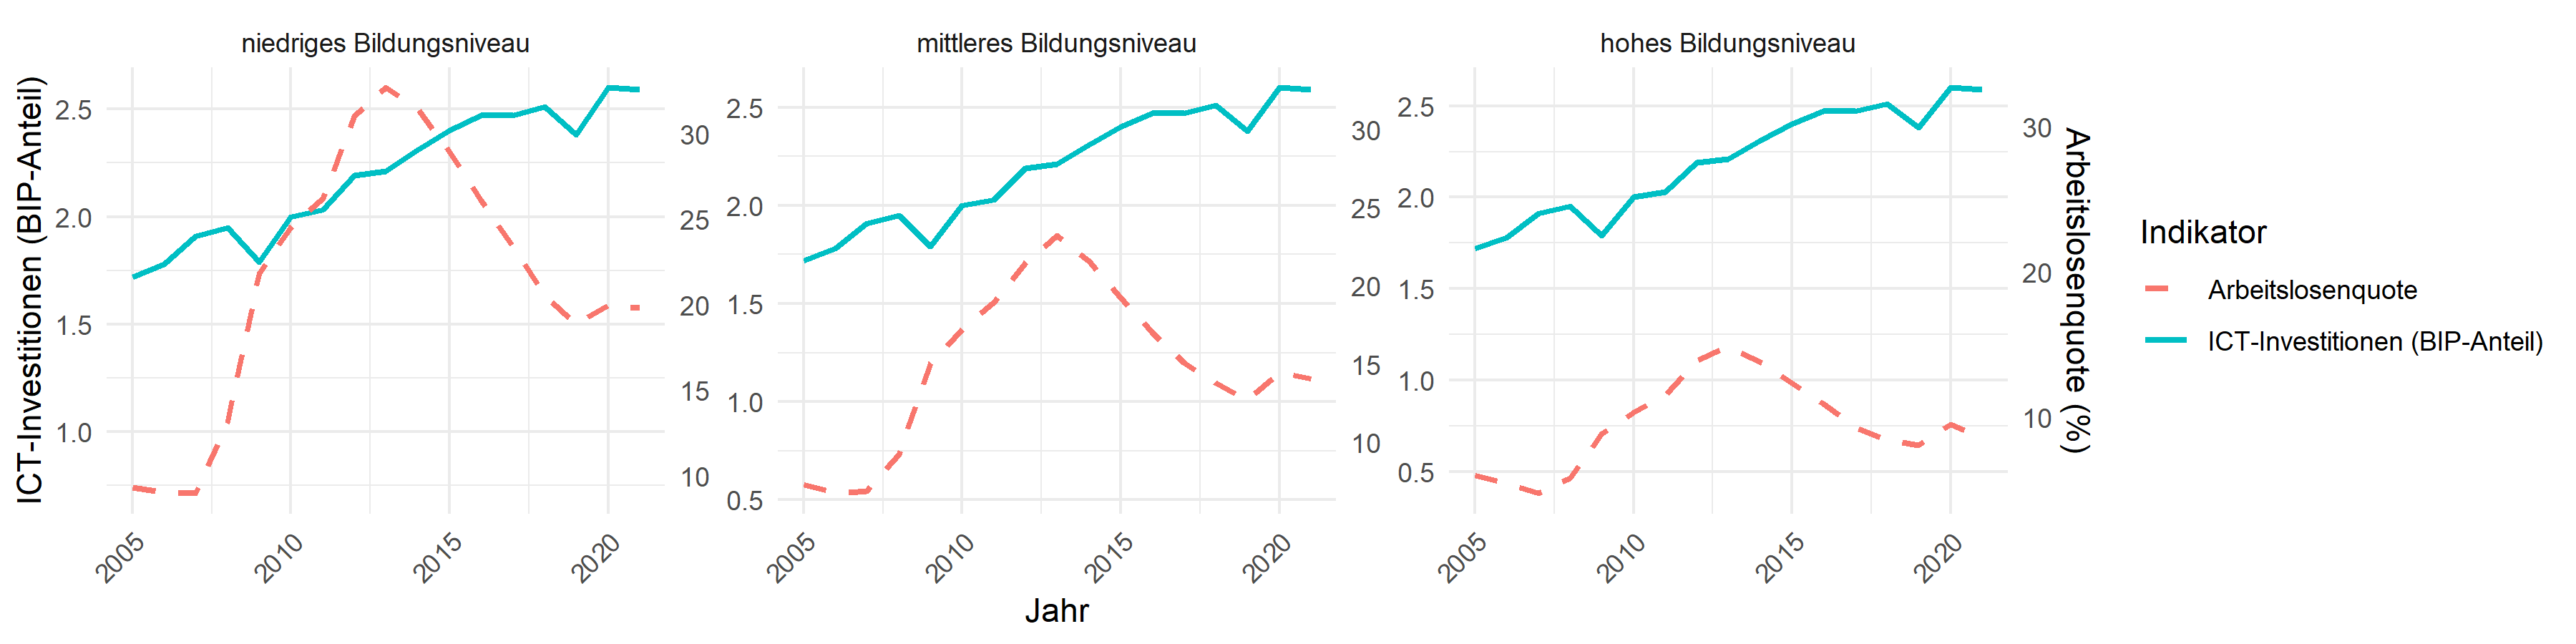
\includegraphics[width=\textwidth]{assets/plot_spain_final.png}
    \caption{Überblick über \textit{\ac{ICT}-Investitionen} und Arbeitslosenquote in 
    Spanien}
    \label{fig:spain}
\end{figure}

Die Abbildung zeigt die Entwicklung der \textit{\ac{ICT}-Investitionen} als Anteil am 
BIP sowie die Arbeitslosenquote in Spanien zwischen 2005 und 2022, differenziert nach 
Bildungsniveau - Spanien steht hier repräsentativ für südeuropäische Wohlfahrtsstaaten. 
Am Beispiel Spaniens ist ein besonders markanter Anstieg der Arbeitslosenquote während 
der Finanz- und Wirtschaftskrise von 2008 bis 2013 zu beobachten. Während die 
\textit{\ac{ICT}-Investitionen} einen insgesamt moderaten Anstieg über den gesamten 
Zeitraum hinweg zeigen, lassen sich drastische Schwankungen in der Arbeitslosenquote 
identifizieren, insbesondere bei Personen mit niedrigem und mittlerem Bildungsniveau.

Bei Personen mit einem niedrigen Bildungsniveau zeigt sich zwischen 2005 und 2008 
eine relativ stabile Arbeitslosenquote von knapp unter 10\%. Ab 2008 kam es jedoch zu 
einem rasanten Anstieg, der bis 2013 einen Höchststand von über 30\% erreichte. Erst 
nach 2013 begann ein kontinuierlicher Rückgang, der sich bis 2020 auf etwa 20\% 
fortsetzte, bevor ein erneuter leichter Anstieg zu beobachten ist. Die 
\textit{\ac{ICT}-Investitionen} entwickelten sich hingegen gleichmäßiger. Sie begannen 
auf einem niedrigen Niveau von etwa 1,75\% des BIP, zeigten nach der Finanzkriese ab 
2010 eine Aufwärtstendenz und stabilisierten sich nach 2015 bei etwa 2,5\%. Der 
Rückgang der Arbeitslosenquote nach 2013 verlief jedoch unabhängig von einer abrupten 
Zunahme der \textit{\ac{ICT}-Investitionen}, was darauf hindeutet, dass 
makroökonomische Faktoren (z. B. wirtschaftliche Erholung, Beschäftigungsprogramme) 
für die Senkung der Arbeitslosigkeit eine zentrale Rolle spielten.

Bei Personen mit mittlerem Bildungsniveau zeigt sich ein sehr ähnlicher Verlauf. Die 
Arbeitslosenquote lag 2005 noch unter 8\%, stieg im Zuge der Wirtschaftskrise bis 2013 
jedoch auf über 20\% an. Erst ab 2014 begann ein deutlicher Rückgang, der sich bis 
2020 auf etwa 10\% fortsetzte. Die \textit{\ac{ICT}-Investitionen} folgten hier einem 
vergleichbaren Muster wie in der Gruppe der gering Qualifizierten, wobei ein leichter, 
aber kontinuierlicher Anstieg sichtbar ist. Dennoch ist keine direkte Korrelation 
zwischen dem Verlauf der \textit{\ac{ICT}-Investitionen} und der Arbeitslosenquote 
ersichtlich, da der massive Anstieg und der spätere Rückgang der Arbeitslosigkeit 
primär durch die wirtschaftliche Entwicklung und nicht durch technologische 
Investitionen bedingt zu sein scheinen.

Bei Personen mit hohem Bildungsniveau war die Arbeitslosenquote insgesamt niedriger, 
zeigte jedoch ebenfalls einen deutlichen Anstieg während der Wirtschaftskrise. Im Jahr 
2005 lag sie unter 5\%, erreichte 2013 jedoch fast 15\%. Danach setzte auch hier ein 
Rückgang ein, und bis 2020 fiel die Quote auf etwa 5\% zurück. Im Gegensatz zu den 
anderen Bildungsgruppen scheinen sich hier die \textit{\ac{ICT}-Investitionen} und 
die Arbeitslosenquote teilweise gegenläufig zu entwickeln. Während die 
\textit{\ac{ICT}-Investitionen} nach 2010 eine stetige Steigerung zeigen und nach 
2015 stabil auf etwa 2,5\% des BIP bleiben, geht die Arbeitslosenquote in derselben 
Phase zurück. Dies könnte darauf hindeuten, dass hochqualifizierte Arbeitskräfte in 
Spanien stärker von der Digitalisierung profitieren konnten als Personen mit 
niedrigerem Bildungsstand.

Spanien als südeuropäischer Wohlfahrtsstaat ist durch einen stark segmentierten 
Arbeitsmarkt gekennzeichnet, der sich durch hohe Anteile an befristeten 
Beschäftigungsverhältnissen sowie eine geringere Arbeitsplatzsicherheit auszeichnet 
\parencite[vgl.][159–160]{bentolila2012two}. Dies könnte eine Erklärung für die starken 
Schwankungen der Arbeitslosenquote im Zuge der Finanzkrise sein, da insbesondere 
gering und mittel Qualifizierte von Entlassungen betroffen waren. Die 
\textit{\ac{ICT}-Investitionen} scheinen langfristig zwar leicht anzusteigen, doch zeigt 
sich kein direkter Zusammenhang zwischen diesen Investitionen und der Arbeitslosenquote 
in den jeweiligen Bildungsgruppen. Vielmehr deutet die Entwicklung darauf hin, dass der 
Arbeitsmarkt in Spanien stark konjunkturabhängig ist und die wirtschaftliche Erholung 
nach 2013 die wichtigste Triebkraft für die Reduktion der Arbeitslosigkeit war 
\parencite[vgl.][157–159]{bentolila2012two}.

Zusammenfassend zeigen die Daten für Spanien eine enge Verbindung zwischen der 
Finanzkrise und den massiven Schwankungen der Arbeitslosenquote, insbesondere bei 
gering und mittel Qualifizierten. Während \textit{\ac{ICT}-Investitionen} über den 
Zeitraum hinweg einen kontinuierlichen, aber moderaten Anstieg zeigen, sind ihre 
direkten Auswirkungen auf die Arbeitslosigkeit unklar. Es könnte jedoch sein, dass 
insbesondere Hochqualifizierte von den steigenden \textit{\ac{ICT}-Investitionen} 
profitieren konnten, während gering Qualifizierte eher von konjunkturellen 
Faktoren abhängig waren.

% Deskriptive Analyse: Grafik "Polen"
\begin{figure}[htbp]
    \centering
    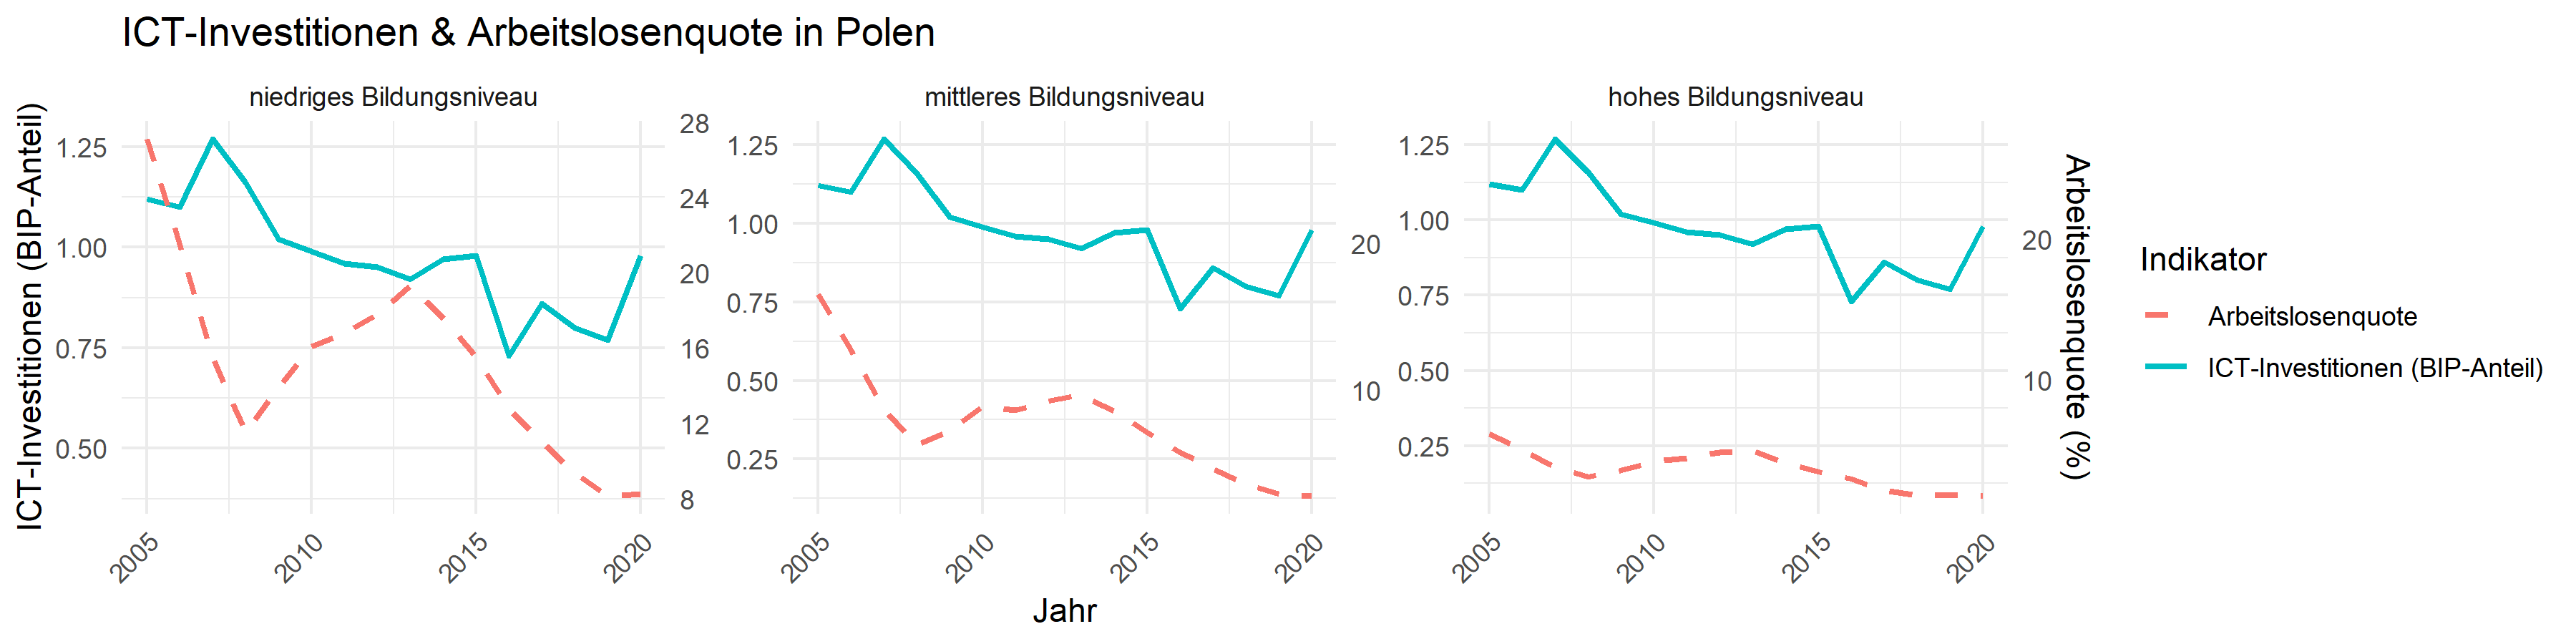
\includegraphics[width=\textwidth]{assets/plot_poland_final.png}
    \caption{Überblick über \textit{\ac{ICT}-Investitionen} und Arbeitslosenquote 
    in Polen}
    \label{fig:poland}
\end{figure}

Die Abbildung zeigt die Entwicklung der \textit{\ac{ICT}-Investitionen} als Anteil 
am BIP sowie die Arbeitslosenquote in Polen zwischen 2005 und 2022 differenziert 
nach Bildungsniveau - Polen steht hier repräsentativ für postsozialistische 
Wohlfahrtsstaaten.

Auffällig ist der durchgängige Rückgang der Arbeitslosenquote in allen 
Bildungsgruppen, während die \textit{\ac{ICT}-Investitionen} über weite Strecken 
konstant bleiben, beziehungsweise sogar ebenfalls einen Rückgang verzeichnen. Dies 
deutet darauf hin, dass makroökonomische oder arbeitsmarktpolitische Faktoren für 
den Rückgang der Arbeitslosigkeit maßgeblich verantwortlich sein könnten.

Bei Personen mit einem niedrigen Bildungsniveau lag die Arbeitslosenquote im Jahr 
2005 bei knapp 28\%. In den darauffolgenden Jahren kam es zu einem raschen Rückgang, 
wobei jedoch zwischen 2010 und 2015 eine Stagnation mit einem kurzen Anstieg auf fast 
20\% zu beobachten ist. Nach 2015 setzte sich der Rückgang der Arbeitslosenquote 
fort, sodass sie bis 2020 auf 8\% fiel. Die \textit{\ac{ICT}-Investitionen} blieben 
über den gesamten Zeitraum hinweg weitgehend konstant und bewegten sich um die 1\% des 
BIP, mit einem leichten Rückgang zwischen 2010 und 2015. Dies deutet darauf hin, dass  
der starke Rückgang der Arbeitslosigkeit nicht direkt mit den 
\textit{\ac{ICT}-Investitionen} zusammenhängt, sondern durch andere wirtschaftliche 
Faktoren beeinflusst wurde, beispielsweise durch eine allgemeine wirtschaftliche 
Stabilisierung nach dem EU-Beitritt Polens und steigende Beschäftigungsmöglichkeiten 
in arbeitsintensiven Branchen.

Für Personen mit einem mittleren Bildungsniveau zeigt sich ein ähnliches Muster, wenn 
auch auf einem insgesamt niedrigeren Ausgangsniveau der Arbeitslosenquote. Während 
diese 2005 noch über 10\% lag, sank sie in den darauffolgenden Jahren rasch auf etwa 
3\% bis 2015 und weiter unter 2\% bis 2020. Zwischen 2010 und 2015 ist jedoch eine 
leichte Erhöhung der Arbeitslosenquote erkennbar, bevor der Trend weiter nach unten 
verlief. Der Rückgang der Arbeitslosigkeit erfolgt weitgehend unabhängig von der 
Entwicklung der \textit{\ac{ICT}-Investitionen}, was darauf hindeutet, dass 
makroökonomische Faktoren wie die Industrialisierung und eine steigende Nachfrage 
nach Arbeitskräften mit mittlerer Qualifikation eine bedeutendere Rolle gespielt 
haben könnten.

Für Personen mit einem hohen Bildungsniveau war die Arbeitslosenquote bereits 
2005 relativ niedrig, lag aber dennoch bei etwa 6\%, was im Vergleich zu anderen 
europäischen Ländern eher hoch ist. Dies könnte auf strukturelle Faktoren des 
polnischen Arbeitsmarktes zurückzuführen sein, wie eine geringere Anzahl 
hochqualifizierter Beschäftigungsmöglichkeiten in den frühen 2000er-Jahren. In den 
darauffolgenden Jahren fiel die Arbeitslosenquote jedoch deutlich und lag bereits 
2015 unter 2\%. Auffällig ist, dass die \textit{\ac{ICT}-Investitionen} in dieser 
Gruppe im Gegensatz zu den anderen Bildungsgruppen eine leichte Steigerung zeigen. 
In der ersten Hälfte des Beobachtungszeitraums bewegten sich die 
\textit{\ac{ICT}-Investitionen} um 1,2\% des BIP, während sie in den Jahren nach 
2015 tendenziell anstiegen. Dies könnte darauf hindeuten, dass der polnische 
Arbeitsmarkt mit steigendem ICT-Investitionsanteil zunehmend hochqualifizierte 
Beschäftigungsmöglichkeiten geschaffen hat. Dennoch bleibt die Kausalität unklar, 
da die Arbeitslosenquote in dieser Gruppe bereits gefallen war, bevor der leichte 
Anstieg der \textit{\ac{ICT}-Investitionen} einsetzte.

Polen als postsozialistischer Wohlfahrtsstaat hat in den letzten Jahrzehnten einen 
tiefgreifenden wirtschaftlichen Wandel durchlaufen. Der EU-Beitritt im Jahr 2004 
führte zu verstärkten ausländischen Direktinvestitionen, einer zunehmenden 
Integration in europäische Produktionsnetzwerke sowie einer generellen 
Modernisierung der Wirtschaft. Diese Entwicklungen spiegeln sich auch in der 
Reduktion der Arbeitslosigkeit wider, die in allen Bildungsgruppen signifikant 
gesunken ist. Besonders bei Personen mit mittlerem und niedrigem Bildungsniveau 
könnte die Expansion von Industriejobs sowie der Dienstleistungssektor eine 
wesentliche Rolle gespielt haben \parencite[vgl.][S. 455–459]{myant2013transition}.

Insgesamt zeigt die Abbildung, dass die Arbeitslosenquote in allen Bildungsgruppen 
stark gesunken ist, während die \textit{\ac{ICT}-Investitionen} nur moderate 
Schwankungen aufweisen. Dies deutet darauf hin, dass die Haupttreiber der 
Beschäftigungsentwicklung in Polen eher in wirtschaftlichen und 
arbeitsmarktpolitischen Veränderungen zu suchen sind als in den direkten 
Auswirkungen von \textit{\ac{ICT}-Investitionen}. Dennoch könnte die leichte 
Zunahme der \textit{\ac{ICT}-Investitionen} im späteren Beobachtungszeitraum 
darauf hinweisen, dass sich der polnische Arbeitsmarkt allmählich in Richtung 
einer wissensbasierten Wirtschaft entwickelt, in der besonders Hochqualifizierte 
profitieren.

% Deskriptive Analyse: Grafik "Schweden"
\begin{figure}[htbp]
    \centering
    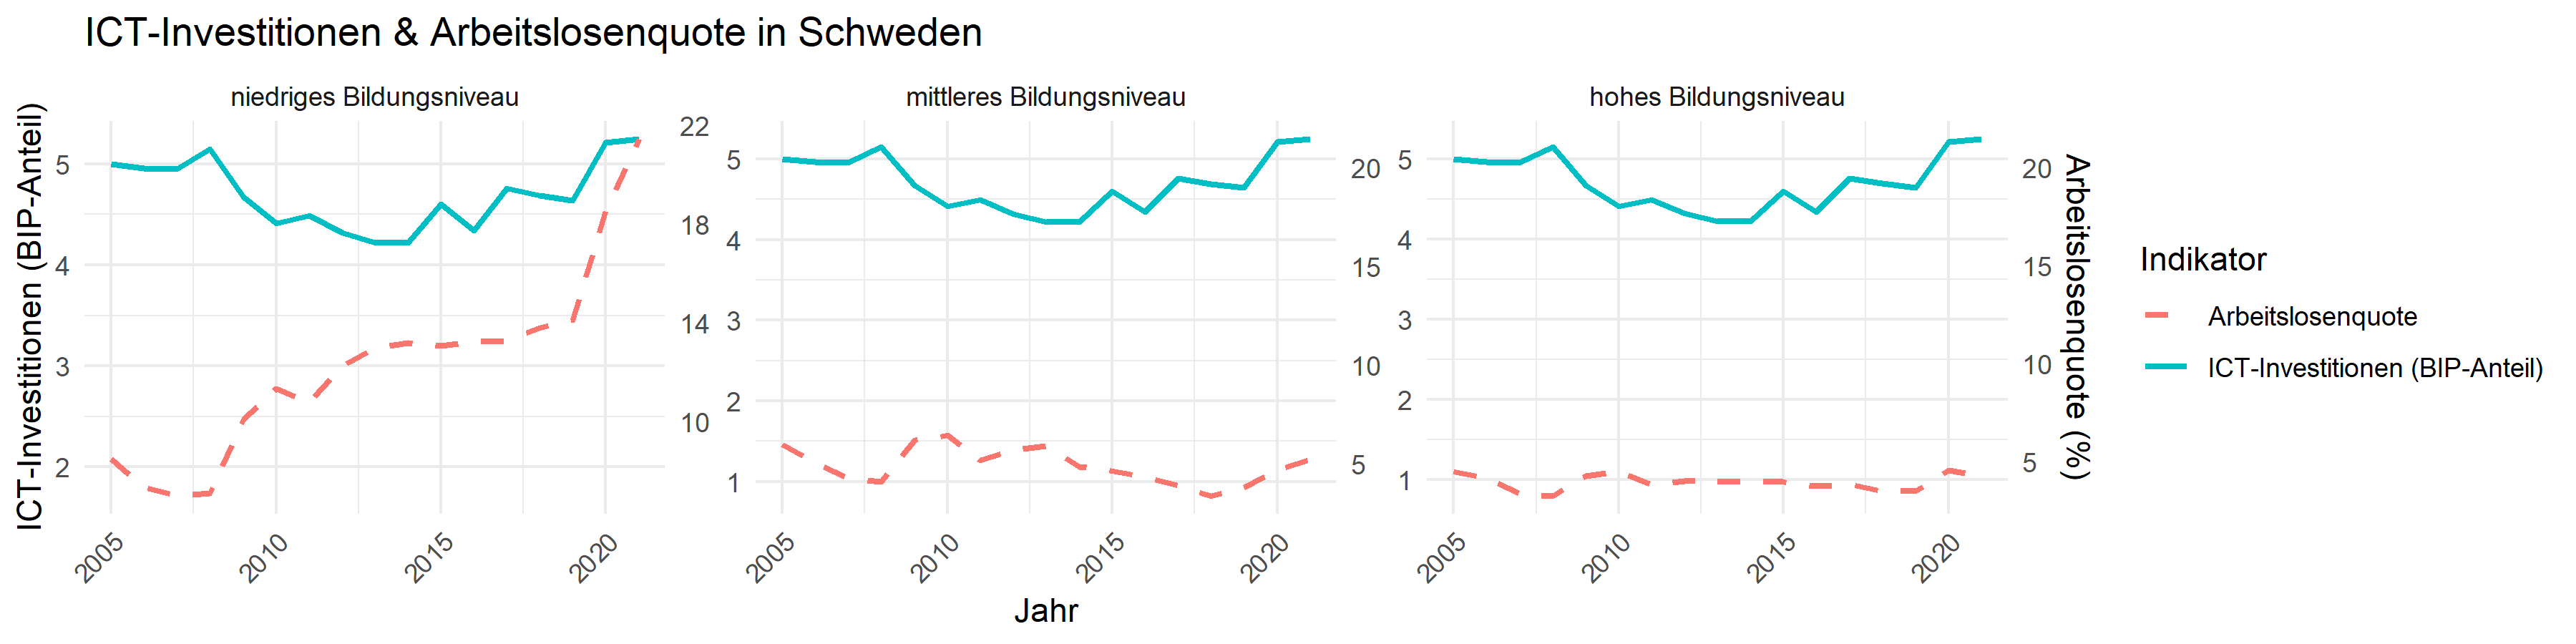
\includegraphics[width=\textwidth]{assets/plot_sweden_final.png}
    \caption{Überblick über \textit{\ac{ICT}-Investitionen} und Arbeitslosenquote in 
    Schweden}
    \label{fig:sweden}
\end{figure}

Die Abbildung zeigt die Entwicklung der \textit{\ac{ICT}-Investitionen} als Anteil 
am BIP sowie die Arbeitslosenquote in Schweden zwischen 2005 und 2022, differenziert 
nach Bildungsniveau - Schweden steht hier repräsentativ für nordische 
Wohlfahrtsstaaten. Im Gegensatz zu anderen Ländern ist hier eine relativ stabile 
Entwicklung der Arbeitslosenquote über den gesamten Zeitraum zu beobachten, mit nur 
moderaten Schwankungen. Auffällig ist zudem, dass die \textit{\ac{ICT}-Investitionen} 
in Schweden im internationalen Vergleich auf einem vergleichsweise hohen Niveau liegen. 
Während sie in der ersten Dekade leichte Schwankungen zeigen, bleibt ihr Niveau ab 
2010 weitgehend konstant und steigt gegen Ende des Betrachtungszeitraums leicht an.

Bei Personen mit einem niedrigen Bildungsniveau lag die Arbeitslosenquote 2005 bei knapp 
5\% und zeigte bis etwa 2010 einen moderaten Anstieg. Nach 2010 stabilisierte sich die 
Arbeitslosenquote zunächst, bevor sie ab 2015 einen erneuten Aufwärtstrend verzeichnete. 
Besonders auffällig ist der deutliche Anstieg nach 2018, der sich bis 2022 fortsetzt. 
Während die Arbeitslosenquote für gering Qualifizierte also in den letzten Jahren 
gestiegen ist, sind die \textit{\ac{ICT}-Investitionen} im selben Zeitraum weitgehend 
stabil geblieben, wenn auch mit einer leicht positiven Tendenz. Dies könnte darauf 
hindeuten, dass die fortschreitende Digitalisierung möglicherweise die 
Beschäftigungsmöglichkeiten für niedrig qualifizierte Arbeitskräfte verschlechtert hat, 
indem sie bestimmte Arbeitsplätze verdrängte oder die Anforderungen an digitale 
Kompetenzen erhöhte - wahrscheinlich hängt diese Beobachtung aber eher mit der 
Corona-Pandemie zusammen.

Für Personen mit einem mittleren Bildungsniveau zeigt sich ein stabiles Muster, mit 
einer weitgehend konstanten Arbeitslosenquote zwischen 2005 und 2018. Während die 
Arbeitslosigkeit 2005 bei unter 5\% lag, gab es bis 2015 eine leichte Abwärtsbewegung, 
gefolgt von einer weitgehenden Stabilisierung. Nach 2018 zeigt sich eine leicht steigende 
Tendenz der Arbeitslosenquote, wenn auch weniger ausgeprägt als bei den gering 
Qualifizierten. Die \textit{\ac{ICT}-Investitionen} sind in dieser Gruppe durchgängig 
hoch und zeigen eine stabile Entwicklung mit leichten Schwankungen. Anders als bei den 
gering Qualifizierten ist hier keine klare gegenläufige Entwicklung zwischen 
\textit{\ac{ICT}-Investitionen} und Arbeitslosigkeit zu erkennen, was darauf hindeutet, 
dass mittlere Qualifikationen in Schweden weniger stark von den technologischen 
Veränderungen betroffen sind.

Bei Personen mit einem hohen Bildungsniveau zeigt sich über den gesamten Zeitraum 
hinweg eine extrem niedrige Arbeitslosenquote. Bereits 2005 lag sie unter 5\% und blieb 
über den gesamten Zeitraum stabil, mit nur minimalen Schwankungen. Auffällig ist, dass 
die \textit{\ac{ICT}-Investitionen} in dieser Gruppe im internationalen Vergleich sehr 
hoch sind, mit Werten, die konstant bei 4-5\% des \ac{BIP} liegen. Die Kombination aus 
hoher \ac{ICT}-Investition und niedriger Arbeitslosenquote deutet darauf hin, dass 
hochqualifizierte Arbeitskräfte in Schweden stark von der Digitalisierung profitieren 
konnten. Dies entspricht auch theoretischen Erwartungen, da hochqualifizierte 
Beschäftigte in wissensintensiven Branchen tätig sind, die von technologischen 
Innovationen profitieren.

Die stabilen \textit{\ac{ICT}-Investitionen} und die insgesamt niedrigen Arbeitslosenquoten 
deuten darauf hin, dass der schwedische Arbeitsmarkt relativ widerstandsfähig gegenüber 
technologischen Veränderungen ist. Allerdings lässt sich bei niedrig qualifizierten 
Arbeitskräften ein Anstieg der Arbeitslosigkeit nach 2018 beobachten, der 
möglicherweise mit strukturellen Veränderungen auf dem Arbeitsmarkt zusammenhängt. 
Dies könnte darauf hindeuten, dass bestimmte Berufe durch die Digitalisierung 
zunehmend verdrängt werden oder dass sich die Anforderungen an digitale Kompetenzen 
verstärkt haben, sodass Geringqualifizierte Schwierigkeiten haben, sich an die 
veränderten Bedingungen anzupassen.

Insgesamt zeigt die Abbildung, dass Schweden ein stabiles Beschäftigungsniveau über 
den gesamten Zeitraum hinweg aufweist, wobei die \textit{\ac{ICT}-Investitionen} 
konstant hoch sind. Während Hoch- und Mittelqualifizierte weitgehend von den 
Entwicklungen profitieren konnten, scheint sich für gering Qualifizierte in den 
letzten Jahren eine Verschlechterung der Beschäftigungssituation abzuzeichnen. Dies 
könnte darauf hindeuten, dass Digitalisierung in hochentwickelten Volkswirtschaften 
wie Schweden zunehmend zu einer Polarisierung des Arbeitsmarktes führt, bei der 
Hochqualifizierte von den Investitionen profitieren, während gering Qualifizierte 
zunehmend unter Druck geraten.

% Deskriptive Analyse: Grafik "Deutschland"
\begin{figure}[htbp]
    \centering
    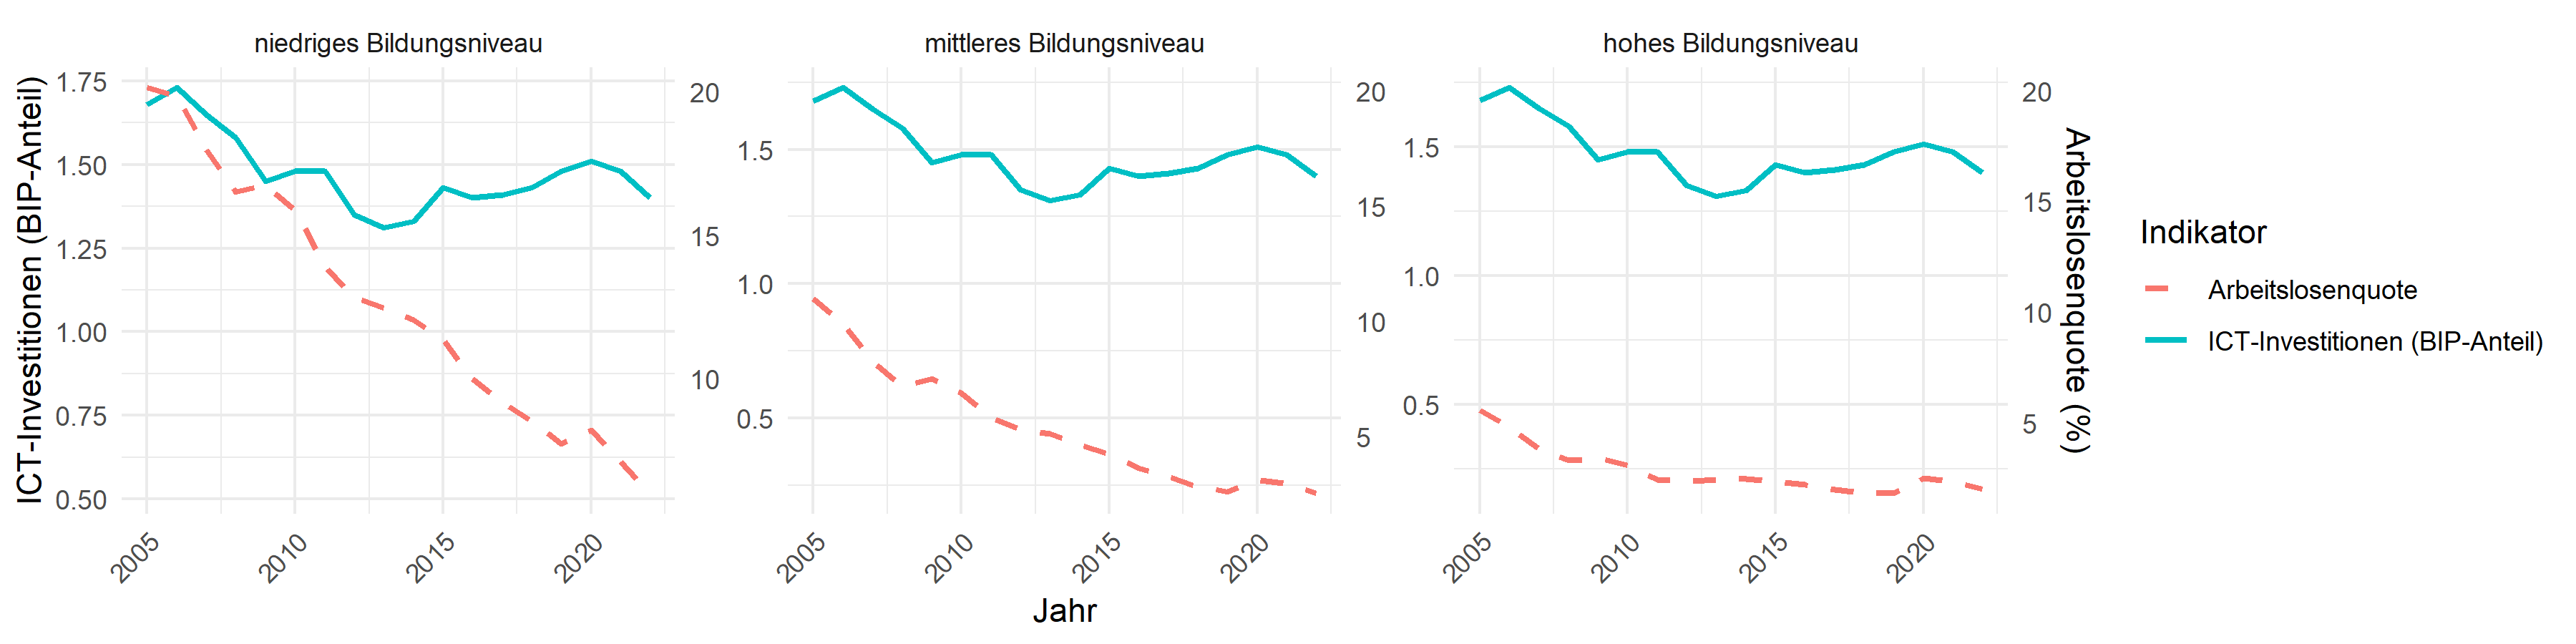
\includegraphics[width=\textwidth]{assets/plot_germany_final.png}
    \caption{Überblick über \textit{\ac{ICT}-Investitionen} und Arbeitslosenquote in 
    Deutschland}
    \label{fig:germany}
\end{figure}

Die Abbildung zeigt die Entwicklung der \textit{\ac{ICT}-Investitionen} als Anteil 
am BIP sowie die Arbeitslosenquote in Deutschland zwischen 2005 und 2022, 
differenziert nach Bildungsniveau - Deutschland steht hier repräsentativ für 
mitteleuropäische Wohlfahrtsstaaten. Dabei lassen sich klare Unterschiede zwischen 
den drei betrachteten Gruppen - niedriges, mittleres und hohes Bildungsniveau - sowohl 
hinsichtlich des Niveaus als auch der Veränderung der Arbeitslosenquoten erkennen. 
Insgesamt zeigen sich über den gesamten Zeitraum hinweg deutliche Rückgänge in der 
Arbeitslosenquote, während die \textit{\ac{ICT}-Investitionen} eine weitgehend 
stabile Entwicklung aufweisen.

Für Personen mit einem niedrigen Bildungsniveau zeigt sich eine besonders hohe 
Arbeitslosenquote zu Beginn des Beobachtungszeitraums, die 2005 bei über 18\% lag. 
In den darauffolgenden Jahren kam es zu einem kontinuierlichen Rückgang, der bis 2020 
Werte unter 5\% erreichte. Diese Entwicklung spiegelt die allgemeine Verbesserung des 
deutschen Arbeitsmarktes wider, insbesondere durch wirtschaftlichen Aufschwung und 
Reformen im Rahmen der Agenda 2010. Die \textit{\ac{ICT}-Investitionen} verzeichneten 
zwischen 2005 und 2010 zunächst einen leichten Rückgang, bevor sie sich um die 1,5\% 
des BIP stabilisierten. Ein direkter Zusammenhang zwischen 
\textit{\ac{ICT}-Investitionen} und der sinkenden Arbeitslosenquote ist nicht 
ersichtlich, da der Rückgang der Arbeitslosenquote bereits vor der leichten 
Stabilisierung der Investitionen begann.

Bei Personen mit mittlerem Bildungsniveau zeigt sich ein ähnliches Muster, wenn auch 
auf einem insgesamt niedrigeren Ausgangsniveau der Arbeitslosenquote. Während diese 
2005 noch bei etwa 10\% lag, fiel sie bis 2020 auf rund 3\% und blieb seither 
weitgehend stabil. Die \textit{\ac{ICT}-Investitionen} zeigen eine konstante 
Entwicklung mit geringen Schwankungen. Auch hier bleibt der direkte Zusammenhang 
zwischen den \textit{\ac{ICT}-Investitionen} und der Arbeitslosenquote unklar, da 
der Rückgang der Arbeitslosigkeit langfristig verläuft und nicht direkt mit den 
Investitionen korreliert.

Für Personen mit hohem Bildungsniveau zeigt sich über den gesamten Zeitraum hinweg 
eine sehr niedrige Arbeitslosenquote. Bereits 2005 lag sie unter 5\% und sank bis
2010 auf unter 2\%, wo sie anschließend auf diesem niedrigen Niveau stabil blieb. 
Im Vergleich zu den anderen Bildungsgruppen weist diese Gruppe somit die geringsten 
Schwankungen auf. Die \textit{\ac{ICT}-Investitionen} zeigen auch hier eine 
weitgehend stabile Entwicklung. Dies könnte darauf hindeuten, dass Hochqualifizierte 
vermehrt in Berufen tätig sind, die von steigenden \textit{\ac{ICT}-Investitionen} 
profitieren, jedoch bleibt auch hier die Kausalität unklar.

Deutschland als konservativer Wohlfahrtsstaat zeichnet sich durch eine enge Verzahnung 
von Bildungssystem und Arbeitsmarkt aus \parencite[vgl.][S. 21–22]{hall2001varieties}. 
Insbesondere das duale Ausbildungssystem und gezielte arbeitsmarktpolitische Maßnahmen 
könnten eine Rolle beim Rückgang der 
Arbeitslosenquoten in den niedrigen und mittleren Bildungsgruppen gespielt haben. 
Die \textit{\ac{ICT}-Investitionen} zeigen über den Beobachtungszeitraum hinweg keine 
drastischen Veränderungen, was darauf hindeutet, dass technologische Entwicklungen 
schrittweise in den Arbeitsmarkt integriert wurden. Besonders für Hochqualifizierte 
könnte eine steigende Nachfrage nach digitalen Fähigkeiten eine Rolle gespielt 
haben, während bei den niedrigen und mittleren Bildungsniveaus der 
Arbeitsmarktrückgang vermutlich durch andere makroökonomische Faktoren beeinflusst 
wurde.

Die Abbildung verdeutlicht insgesamt, dass die Arbeitslosenquoten in allen 
Bildungsgruppen über die Jahre hinweg gesunken sind, während die 
\textit{\ac{ICT}-Investitionen} vergleichsweise stabil geblieben sind. Dies lässt darauf 
schließen, dass der Rückgang der Arbeitslosigkeit nicht direkt durch 
\textit{\ac{ICT}-Investitionen} getrieben wurde, sondern eher mit makroökonomischen 
Entwicklungen und strukturellen Veränderungen auf dem deutschen Arbeitsmarkt 
zusammenhängt.

% Deskriptive Analyse: Grafik "Großbritannien"
\begin{figure}[htbp]
    \centering
    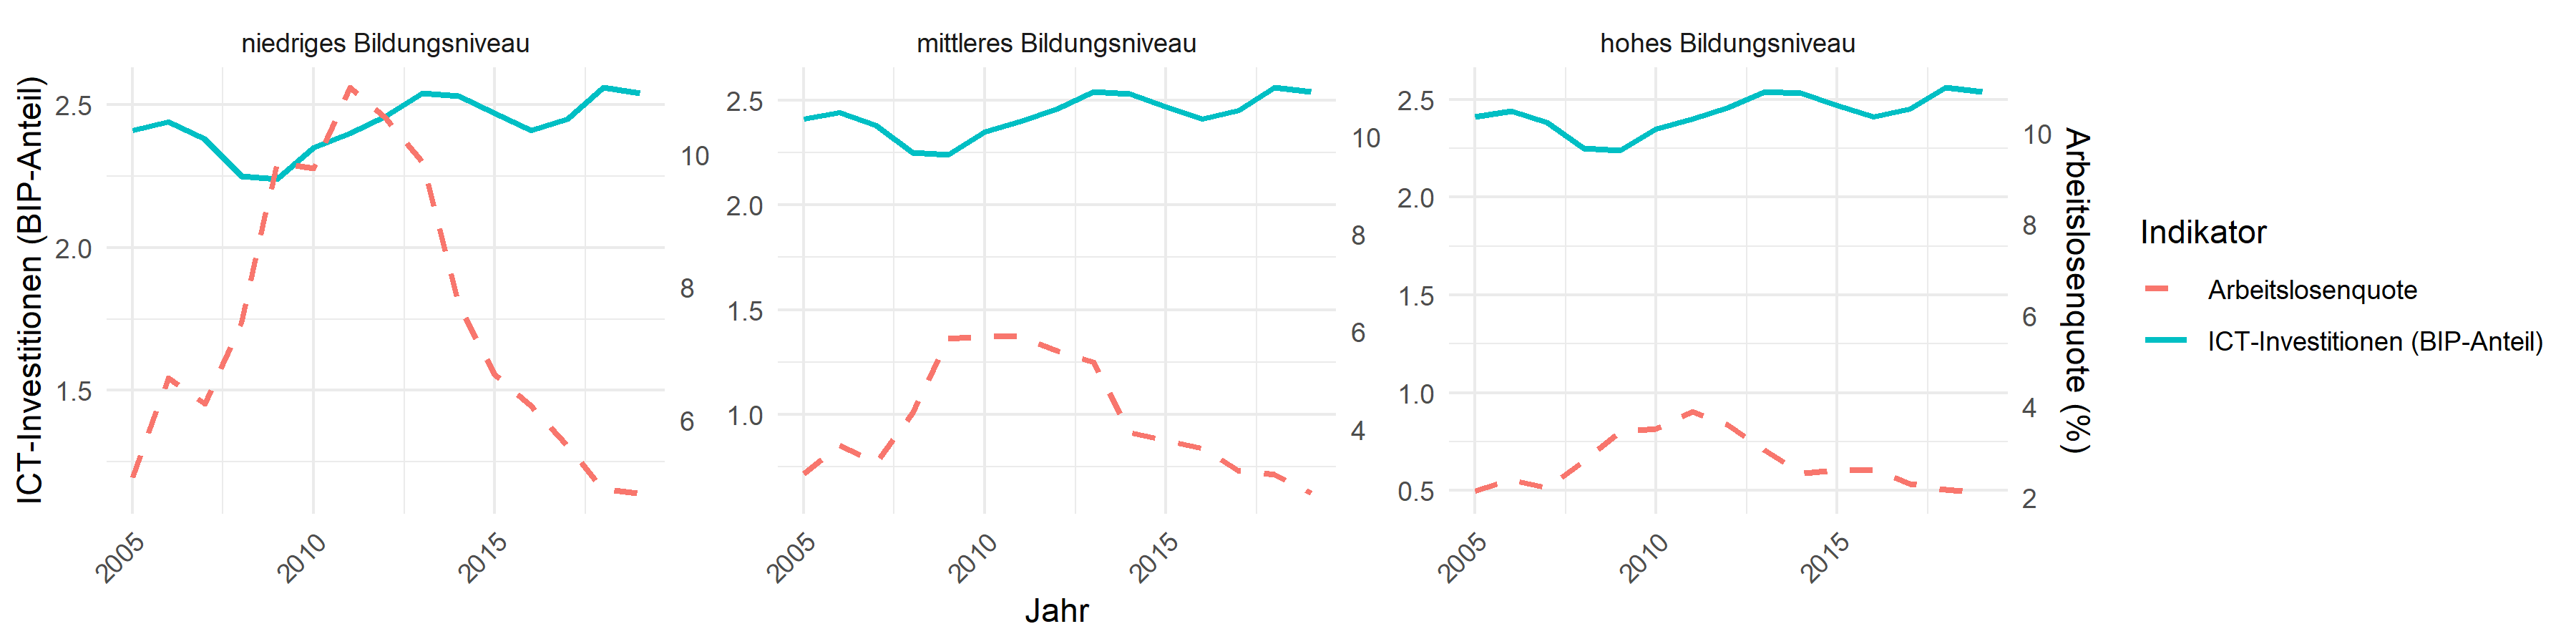
\includegraphics[width=\textwidth]{assets/plot_uk_final.png}
    \caption{Überblick über \textit{\ac{ICT}-Investitionen} und Arbeitslosenquote in 
    Großbritannien}
    \label{fig:uk}
\end{figure}

Die Abbildung zeigt die Entwicklung der \textit{\ac{ICT}-Investitionen} als Anteil am BIP 
sowie die Arbeitslosenquote in Großbritannien zwischen 2005 und 2022, differenziert nach 
Bildungsniveau - Großbritannien steht hier repräsentativ für angelsächsische 
Wohlfahrtsstaaten. Im Vergleich zu anderen Wohlfahrtsstaatentypen weist Großbritannien eine 
relativ konstante Arbeitslosenquote auf, die über den Zeitraum hinweg nur leichte 
Rückgänge zeigt. Auffällig ist, dass die \textit{\ac{ICT}-Investitionen} in Großbritannien 
zwar einen moderaten Anstieg aufweisen, sich jedoch auf einem relativ niedrigen Niveau 
bewegen.

Bei Personen mit einem niedrigen Bildungsniveau lag die Arbeitslosenquote im Jahr 2005 
bei etwa 8\% und sank bis 2020 auf unter 4\%. Anders als in Ländern mit stärker 
regulierten Arbeitsmärkten zeigt sich hier kein abrupter Rückgang, sondern eine 
schrittweise Anpassung über den Zeitraum hinweg. Gleichzeitig zeigen die 
\textit{\ac{ICT}-Investitionen} einen leicht steigenden Trend, bleiben jedoch im Bereich 
von etwa 1,5\% des BIP. Ein klarer Zusammenhang zwischen \textit{\ac{ICT}-Investitionen} 
und der Arbeitslosenquote lässt sich nicht unmittelbar erkennen, was darauf hindeuten 
könnte, dass andere arbeitsmarktpolitische oder wirtschaftliche Faktoren maßgeblicher für 
die Reduktion der Arbeitslosigkeit sind.

Bei Personen mit mittlerem Bildungsniveau zeigt sich ein ähnliches Muster. Die 
Arbeitslosenquote lag 2005 bei etwa 6\% und fiel bis 2015 auf rund 3\%, wo sie sich 
anschließend stabilisierte. Die \textit{\ac{ICT}-Investitionen} zeigen hier eine geringe 
Zunahme, bleiben jedoch weitgehend konstant im Bereich von 1,5\% bis 2\% des BIP. Auch in 
dieser Gruppe scheint der Rückgang der Arbeitslosenquote eher mit marktwirtschaftlichen 
Anpassungen als mit direkten Effekten der \textit{\ac{ICT}-Investitionen} zusammenzuhängen. 
Der relativ geringe Anstieg der Investitionen deutet darauf hin, dass die britische 
Wirtschaft zwar technologische Entwicklungen integriert, jedoch nicht in dem Ausmaß wie 
andere hochdigitalisierte Volkswirtschaften.

Für Personen mit hohem Bildungsniveau zeigt sich über den gesamten Zeitraum hinweg eine 
sehr niedrige Arbeitslosenquote. Bereits 2005 lag sie unter 3\% und blieb über den 
gesamten Zeitraum weitgehend stabil, mit nur minimalen Schwankungen. Die 
\textit{\ac{ICT}-Investitionen} zeigen auch hier eine relativ konstante Entwicklung, 
liegen jedoch ebenfalls im Bereich von 1,5\% bis 2\% des BIP. Dies deutet darauf hin, 
dass Hochqualifizierte kaum von negativen Beschäftigungseffekten durch Digitalisierung 
betroffen sind. Vielmehr könnte der flexible britische Arbeitsmarkt es dieser Gruppe 
erleichtert haben, sich an technologische Veränderungen anzupassen.

Großbritannien als anglo-sächsischer Wohlfahrtsstaat zeichnet sich durch einen 
weniger regulierten Arbeitsmarkt aus, der sich durch eine hohe Flexibilität und eine 
geringere staatliche Intervention auszeichnet \parencite[vgl.][S. 21]{trabert1997entwicklung}. 
Diese Charakteristik könnte erklären, warum die Arbeitslosenquoten über den Zeitraum hinweg 
relativ stabil bleiben und gleichzeitig keine drastischen Veränderungen im Bereich der 
\textit{\ac{ICT}-Investitionen} feststellbar sind. Der moderate Rückgang der Arbeitslosigkeit 
deutet darauf hin, dass sich der britische Arbeitsmarkt schrittweise an Digitalisierung angepasst 
hat, ohne dass bestimmte Gruppen massiv benachteiligt wurden.

Zusammenfassend zeigt die Abbildung, dass sich die britische Arbeitslosenquote über die 
Jahre hinweg in allen Bildungsgruppen verringert hat, wenn auch nicht so drastisch wie in 
anderen Ländern. Gleichzeitig bleiben die \textit{\ac{ICT}-Investitionen} auf einem 
relativ niedrigen Niveau und zeigen keine unmittelbare Korrelation mit den Veränderungen 
der Arbeitslosenquote. Dies deutet darauf hin, dass makroökonomische Faktoren wie die 
Arbeitsmarktflexibilität und allgemeine wirtschaftliche Entwicklung eine wichtigere Rolle 
für die Beschäftigungsdynamik spielen als allein die Höhe der \textit{\ac{ICT}-Investitionen}.


%%%%%%%%%%%%%%%%%%%%%%%%%
% Multivariate Analysen %
%%%%%%%%%%%%%%%%%%%%%%%%%

\subsection{Multivariate Analysen}

% Multivariate Analyse: Einleitung
Die Zusammenfassung der Ergebnisse aus den Modellen mit Kontrollvariablen zeigt eine 
umfassende, jedoch differenzierte Analyse der Auswirkungen von 
\textit{\ac{ICT}-Investitionen} auf die Arbeitslosenquote in den drei Bildungsgruppen 
(„niedriges Bildungsniveau“, „mittleres Bildungsniveau“, „hohes Bildungsniveau“). Die
Modelle liefern wichtige Hinweise auf die Bedeutung makroökonomischer Rahmenbedingungen
und institutioneller Strukturen, während der direkte Einfluss von
\textit{\ac{ICT}-Investitionen} signifikant, aber unterschiedlich stark ausfällt.

% Multivariate Analyse: Modelle ohne Interaktion
% TODO: - (Stand 04.03.2025)

\begin{table}[H]
\caption{Einzelwerte der Regressionsmodellparameter für die Kontrollmodelle}
\resizebox{\textwidth}{!}{
\centering
\begin{talltblr}[         %% tabularray outer open
entry=none,label=none,
note{}={+ p \num{< 0.1}, * p \num{< 0.05}, ** p \num{< 0.01}, *** p \num{< 0.001}},
]                     %% tabularray outer close
{                     %% tabularray inner open
colspec={Q[]Q[]Q[]Q[]},
column{2,3,4}={}{halign=c,},
column{1}={}{halign=l,},
hline{13}={1,2,3,4}{solid, black, 0.05em},
}                     %% tabularray inner close
\toprule
& niedriges
Bildungsniv.
(Kontrolle) & mittleres
Bildungsniv.
(Kontrolle) & hohes
Bildungsniv.
(Kontrolle) \\ \midrule %% TinyTableHeader
ICT\_INVEST\_SHARE\_GDP     & \num{2.302}***  & \num{1.157}***  & \num{0.455}***  \\
& (\num{0.232})   & (\num{0.146})   & (\num{0.086})   \\
GDP\_PER\_CAPITA             & \num{-0.194}*** & \num{-0.153}*** & \num{-0.083}*** \\
& (\num{0.018})   & (\num{0.012})   & (\num{0.007})   \\
PERCENT\_TERTIARY\_EDUCATION & \num{0.606}***  & \num{0.282}***  & \num{0.140}***  \\
& (\num{0.052})   & (\num{0.032})   & (\num{0.019})   \\
REGULATION\_STRICTNESS        & \num{-0.147}    & \num{-0.118}*   & \num{-0.085}*   \\
& (\num{0.094})   & (\num{0.059})   & (\num{0.035})   \\
PERCENT\_EMPLOYEES\_TUD      & \num{0.128}**   & \num{0.106}***  & \num{0.025}+    \\
& (\num{0.039})   & (\num{0.025})   & (\num{0.015})   \\
YEAR\_FACTOR & True & True & True \\
Num.Obs.                       & \num{3973}      & \num{3973}      & \num{3973}      \\
R2                             & \num{0.304}     & \num{0.308}     & \num{0.281}     \\
R2 Adj.                        & \num{0.295}     & \num{0.299}     & \num{0.272}     \\
AIC                            & \num{21393.1}   & \num{17747.2}   & \num{13530.6}   \\
BIC                            & \num{21537.7}   & \num{17891.8}   & \num{13675.2}   \\
RMSE                           & \num{3.55}      & \num{2.25}      & \num{1.32}      \\
\bottomrule
\end{talltblr}
}
\label{tab:models_control}
\end{table}


% Multivariate Analyse: Modell ohne Interaktion (niedriges Bildungsniveau)
Im Modell für die Gruppe mit niedrigem Bildungsniveau zeigt der geschätzte Koeffizient
für \textit{\ac{ICT}-Investitionen} einen positiven Wert von 2,302*** (p < 0,001), was auf
einen signifikanten positiven Zusammenhang zwischen \ac{ICT}-Investitionen und der
Arbeitslosenquote dieser Gruppe hindeutet. Dies bedeutet, dass in Ländern mit
höheren \ac{ICT}-Investitionen die Arbeitslosigkeit unter geringqualifizierten Personen
tendenziell ansteigt. Dies bestätigt die Hypothese, dass gering Qualifizierte stärker von
den negativen Effekten der Digitalisierung betroffen sind.

Das \textit{\ac{BIP} pro Kopf} zeigt mit einem Koeffizienten von -0,194*** (p < 0,001)
einen stark negativen und signifikanten Einfluss. Dies weist darauf hin, dass in wohlhabenderen
Ländern die Arbeitslosenquote für geringqualifizierte Personen tendenziell niedriger ist,
möglicherweise aufgrund eines breiteren Angebots an Beschäftigungsmöglichkeiten oder
arbeitsmarktpolitischer Maßnahmen.

Der \textit{Tertiärer Bildungsanteil} hat einen signifikanten positiven Effekt von 0,606**
(p < 0,01), was darauf hindeutet, dass eine höhere Bildungsbeteiligung in der Gesamtbevölkerung
zu strukturellen Veränderungen des Arbeitsmarktes führt, die auch auf geringqualifizierte Arbeitskräfte
Auswirkungen haben könnten. Die \textit{Gewerkschaftsdichte} weist mit einem Koeffizienten von 0,128**
(p < 0,01) einen signifikanten positiven Zusammenhang auf, was darauf hindeutet, dass eine höhere
gewerkschaftliche Organisationsrate mit einer leicht höheren Arbeitslosenquote für diese Gruppe
einhergeht. Die \textit{Regulierungsstrenge des Arbeitsmarkts} zeigt keinen signifikanten Effekt für
diese Gruppe.

% Multivariate Analyse: Modell ohne Interaktion (mittleres Bildungsniveau)
Für das mittlere Bildungsniveau ergibt sich ebenfalls ein signifikanter positiver Zusammenhang
zwischen \textit{\ac{ICT}-Investitionen} und Arbeitslosigkeit. Der geschätzte Koeffizient beträgt
1,157*** (p < 0,001), was darauf hindeutet, dass höhere \ac{ICT}-Investitionen mit einer steigenden
Arbeitslosigkeit in dieser Gruppe verbunden sind. Dies bestätigt die Hypothese, dass mittelqualifizierte
Arbeitskräfte ebenfalls von negativen Effekten der Digitalisierung betroffen sein können, wenn auch in
gerigerem Maße als geringqualifizierte Personen.

Das \textit{\ac{BIP} pro Kopf} zeigt mit einem Koeffizienten von -0,153*** (p < 0,001) einen signifikanten
negativen Zusammenhang. Dies deutet darauf hin, dass eine höhere Wirtschaftsleistung mit einer geringeren
Arbeitslosenquote für mittelqualifizierte Personen verbunden ist, vermutlich aufgrund eines stabileren
Arbeitsmarktes und größerer Weiterbildungsmöglichkeiten.

Der \textit{Tertiärer Bildungsanteil} weist einen signifikanten positiven Effekt von 0,282**
(p < 0,01) auf, was darauf hindeutet, dass eine höhere tertiäre Bildungsbeteiligung mit strukturellen
Arbeitsmarktveränderungen einhergeht, die möglicherweise den Druck auf mittelqualifizierte Berufe erhöhen.
Die \textit{Gewerkschaftsdichte} zeigt mit einem Koeffizienten von 0,106*** (p < 0,001) eine signifikante
positive Korrelation mit der Arbeitslosenquote, was darauf hindeutet, dass eine stärkere gewerkschaftliche
Organisationsrate nicht zwangsläufig zu niedrigeren Arbeitslosenquoten in dieser Gruppe führt. Die
\textit{Regulierungsstrenge des Arbeitsmarkts} hat einen signifikant negativen Effekt von -0,118*
(p < 0,05), was darauf hindeutet, dass strengere Arbeitsmarktregulierungen für diese Gruppe
stabilisierend wirken könnten, indem sie den Arbeitsplatzverlust für mittelqualifizierte Beschäftigte 
reduzieren.

% Multivariate Analyse: Modell ohne Interaktion (hohes Bildungsniveau)
Für das hohe Bildungsniveau zeigt das Modell einen signifikanten, aber kleineren positiven
Zusammenhang zwischen \textit{\ac{ICT}-Investitionen} und Arbeitslosigkeit. Der Koeffizient beträgt
0,455*** (p < 0,001), was darauf hindeutet, dass auch hochqualifizierte Personen in Ländern mit
höheren \ac{ICT}-Investitionen von einem leichten Anstieg der Arbeitslosenquote betroffen sein
könnten. Dies widerspricht der ursprünglichen Erwartung, dass Hochqualifizierte weniger
von negativen Arbeitsmarkteffekten der Digitalisierung betroffen sind. Eine mögliche Erklärung
könnte darin liegen, dass technologische Entwicklungen auch anspruchsvolle Tätigkeiten
verändern oder ersetzen.

Das \textit{\ac{BIP} pro Kopf} zeigt mit einem Koeffizienten von -0,083*** (p < 0,001)
weiterhin einen signifikant negativen Zusammenhang, was bestätigt, dass wirtschaftlich stärkere
Länder tendenziell geringere Arbeitslosenquoten für Hochqualifizierte aufweisen. Der
\textit{Tertiärer Bildungsanteil} hat mit 0.140*** (p < 0,001) ebenfalls einen signifikant positiven
Zusammenhang. Dies deutet darauf hin, dass ein höherer Anteil an tertiär gebildeten Personen
möglicherweise mit einer steigenden Konkurrenz innerhalb dieser Qualifikationsgruppe verbunden ist.

Die \textit{Gewerkschaftsdichte} hat in dieser Gruppe mit 0.025+ (p < 0,1) einen nur schwach
signifikanten positiven Effekt. Die \textit{Regulierungsstrenge des Arbeitsmarkts} zeigt mit einem
Koeffizienten von -0,085* (p < 0,05) einen signifikant negativen Zusammenhang, was darauf hindeutet,
dass striktere Arbeitsmarktregulierungen möglicherweise schützend für hochqualifizierte Arbeitnehmer
wirken, indem sie Arbeitsplatzsicherheit erhöhen oder Marktzugang regulieren.

% Modellgüte und Interpretation der Ergebnisse
Die Modellgüte variiert zwischen den Bildungsgruppen, wobei die erklärten Varianzen (R²-Werte)
zwischen 27,2\% und 30,8\% der Variation in der Arbeitslosenquote erklären. Im Modell für das
niedrige Bildungsniveau beträgt der R²-Wert 0,304, für das mittlere Bildungsniveau 0,308 und für das hohe
Bildungsniveau 0,272. Diese Werte zeigen, dass die Modelle einen relevanten, aber begrenzten Teil der
Variation erklären können. Der adjustierte R²-Wert liegt bei 0,295 (niedriges Bildungsniveau), 0,299
(mittleres Bildungsniveau) und 0,262 (hohes Bildungsniveau). Diese Werte verdeutlichen, dass weitere
nicht modellierte Einflussfaktoren existieren, die in zukünftigen Studien berücksichtigt werden sollten.

% Fazit der multivariaten Analyse ohne Interaktion
Zusammenfassend zeigen die Modelle mit Kontrollvariablen, dass \textit{\ac{ICT}-Investitionen}
in allen Bildungsgruppen einen signifikanten positiven Einfluss auf die Arbeitslosenquote haben.
Die geschätzten Koeffizienten sind durchweg signifikant (niedriges Bildungsniveau: 2,302***,
mittleres Bildungsniveau: 1,157***, hohes Bildungsniveau: 0,455***), was darauf hindeutet, dass
\ac{ICT}-Investitionen in der derzeitigen Form eher zu einem Anstieg der Arbeitslosigkeit führen.

Die Ergebnisse deuten darauf hin, dass sich die Auswirkungen von Investitionen in \ac{ICT} nicht
ausschließlich auf geringqualifizierte Arbeitnehmer konzentrieren, sondern auch Mittel- und
Hochqualifizierte betreffen können. Besonders für Geringqualifizierte zeigt sich der stärkste
Zusammenhang, was mit bisherigen Annahmen über die Verwundbarkeit dieser Gruppe in digitalen
Arbeitsmärkten übereinstimmt. Gleichzeitig widersprechen die Ergebnisse der Erwartung, dass
Hochqualifizierte von steigenden Investitionen in \ac{ICT} profitieren.

Makroökonomische Faktoren, insbesondere das \textit{\ac{BIP} pro Kopf}, haben in allen Modellen 
einen signifikanten negativen Einfluss auf die Arbeitslosenquote. Dies bestätigt, dass wirtschaftlich 
stärkere Länder tendenziell geringere Arbeitslosenquoten aufweisen. Striktere 
Arbeitsmarktregulierungenzeigen in der Gruppe der Mittel- und Hochqualifizierten negative Effekte auf 
die Arbeitslosigkeit, was darauf hindeutet, dass Regulierung möglicherweise Schutz für diese Gruppen 
bietet. Eine höhere Bildungsbeteiligung zeigt in allen Gruppen einen positiven Zusammenhang mit der 
Arbeitslosenquote, was darauf hindeutet, dass eine verstärkte Tertiärbildung allein nicht ausreicht, 
um Digitalisierungseffekte am Arbeitsmarkt auszugleichen.

Die Erklärungswerte (R²) der Modelle sind moderat (zwischen 0,272 und 0,308), was darauf
hindeutet, dass wesentliche strukturelle und institutionelle Einflussfaktoren erfasst wurden,
aber nicht die gesamte Variation in den Arbeitslosenquoten erklären. Dies zeigt die Notwendigkeit
einer differenzierteren Untersuchung durch Interaktionsmodelle, um die Mechanismen hinter den
beobachteten Zusammenhängen besser zu verstehen.

% Multivariate Analyse: Modelle mit Interaktion
\begin{table}[H]
\caption{Einzelwerte der Regressionsmodellparameter für die Interaktionsmodelle}
\resizebox{\textwidth}{!}{ % Resize to fit the page width
\centering
\begin{talltblr}[         %% tabularray outer open
entry=none,label=none,
note{}={+ p \num{< 0.1}, * p \num{< 0.05}, ** p \num{< 0.01}, *** p \num{< 0.001}},
]                     %% tabularray outer close
{                     %% tabularray inner open
colspec={Q[]Q[]Q[]Q[]},
column{2,3,4}={}{halign=c,},
column{1}={}{halign=l,},
hline{21}={1,2,3,4}{solid, black, 0.05em},
}                     %% tabularray inner close
\toprule
& niedriges
Bildungsniv.
(Interaktion) & mittleres
Bildungsniv.
(Interaktion) & hohes
Bildungsniv.
(Interaktion) \\ \midrule %% TinyTableHeader
ICT\_INVEST\_SHARE\_GDP                                    & \num{4.671}***  & \num{3.246}***  & \num{1.259}***  \\
& (\num{0.572})   & (\num{0.364})   & (\num{0.214})   \\
GDP\_PER\_CAPITA                                            & \num{-0.180}*** & \num{-0.151}*** & \num{-0.083}*** \\
& (\num{0.018})   & (\num{0.012})   & (\num{0.007})   \\
PERCENT\_TERTIARY\_EDUCATION                                & \num{0.619}***  & \num{0.268}***  & \num{0.122}***  \\
& (\num{0.051})   & (\num{0.032})   & (\num{0.019})   \\
REGULATION\_STRICTNESS                                       & \num{-0.152}+   & \num{-0.126}*   & \num{-0.091}**  \\
& (\num{0.092})   & (\num{0.058})   & (\num{0.034})   \\
PERCENT\_EMPLOYEES\_TUD                                     & \num{0.103}**   & \num{0.090}***  & \num{0.014}     \\
& (\num{0.038})   & (\num{0.024})   & (\num{0.014})   \\
ICT\_INVEST\_SHARE\_GDP × WELFARE\_STATECentral European  & \num{0.676}     & \num{-0.647}    & \num{-0.212}    \\
& (\num{0.718})   & (\num{0.456})   & (\num{0.268})   \\
ICT\_INVEST\_SHARE\_GDP × WELFARE\_STATENordic            & \num{0.033}     & \num{-0.443}    & \num{0.639}*    \\
& (\num{0.837})   & (\num{0.532})   & (\num{0.313})   \\
ICT\_INVEST\_SHARE\_GDP × WELFARE\_STATEPost-socialist    & \num{-5.200}*** & \num{-3.579}*** & \num{-1.415}*** \\
& (\num{0.643})   & (\num{0.409})   & (\num{0.240})   \\
ICT\_INVEST\_SHARE\_GDP × WELFARE\_STATESouthern European & \num{1.465}     & \num{-3.066}*** & \num{-2.880}*** \\
& (\num{1.051})   & (\num{0.669})   & (\num{0.393})   \\
YEAR\_FACTOR & True & True & True \\
Num.Obs.                                                      & \num{3973}      & \num{3973}      & \num{3973}      \\
R2                                                            & \num{0.337}     & \num{0.333}     & \num{0.306}     \\
R2 Adj.                                                       & \num{0.327}     & \num{0.324}     & \num{0.297}     \\
AIC                                                           & \num{21212.7}   & \num{17609.6}   & \num{13396.2}   \\
BIC                                                           & \num{21382.5}   & \num{17779.3}   & \num{13566.0}   \\
RMSE                                                          & \num{3.47}      & \num{2.20}      & \num{1.30}      \\
\bottomrule
\end{talltblr}
}
\label{tab:models_interaction}
\end{table}


% Multivariate Analyse: Modelle mit Interaktion
Die Modelle mit Interaktionseffekten und Jahresdummies liefern eine differenziertere Perspektive auf den 
Zusammenhang zwischen \textit{\ac{ICT}-Investitionen} und der \textit{Arbeitslosenquote}. Im Vergleich zu den 
Basis-Modellen ohne Interaktionen zeigen sich hier mehrere signifikante Zusammenhänge, insbesondere mit 
institutionellen Faktoren wie den \textit{Wohlfahrtsstaatentypen}.

Die Interaktionseffekte zwischen \textit{\ac{ICT}-Investitionen} und den \textit{Wohlfahrtsstaatentypen} liefern 
wichtige Erkenntnisse über die Rolle institutioneller Rahmenbedingungen. Da die Referenzkategorie der 
angelsächsische Wohlfahrtsstaat ist, sind die Interaktionseffekte relativ zu diesem Typ zu interpretieren.

Für postsozialistische Wohlfahrtsstaaten zeigen sich die stärksten negativen Interaktionseffekte. Für 
das niedrige Bildungsniveau beträgt der Interaktionseffekt -5,200* (p < 0,001), für das mittlere 
Bildungsniveau -3,579* (p < 0,001) und für das hohe Bildungsniveau -1,415* (p < 0,001). Diese signifikant 
negativen Werte bedeuten, dass die negativen Auswirkungen von \ac{ICT}-Investitionen auf die \textit{Arbeitslosenquote} 
in diesen Ländern geringer ausfallen als in den liberalen Wohlfahrtsstaaten. Da die Interaktionseffekte 
in ihrer absoluten Höhe sogar größer sind als die Haupteffekte der \ac{ICT}-Investitionen, deutet dies darauf 
hin, dass \ac{ICT}-Investitionen in postsozialistischen Staaten nicht zu einer höheren Arbeitslosigkeit 
führen, sondern möglicherweise stabilisierend wirken. Eine mögliche Erklärung hierfür könnte sein, dass 
diese Länder gezielte wirtschaftspolitische Maßnahmen oder strukturelle Besonderheiten aufweisen, die 
negative Effekte der Digitalisierung auf den Arbeitsmarkt abmildern.

Für mitteleuropäische Wohlfahrtsstaaten sind die Interaktionseffekte negativ, aber nicht signifikant. 
Dies bedeutet, dass sich diese Länder nicht signifikant von der Referenzkategorie unterscheiden. Mit 
anderen Worten gibt es keine eindeutigen Belege dafür, dass \ac{ICT}-Investitionen in diesen Ländern 
systematisch andere Auswirkungen auf die Arbeitslosigkeit haben als in den liberalen Wohlfahrtsstaaten. 
Mitteleuropäische Länder wie Deutschland oder Frankreich verfügen über relativ stabile 
Arbeitsmarktstrukturen und ein starkes duales Bildungssystem, das möglicherweise negative Effekte abfedert. 
Allerdings zeigen die Ergebnisse keine signifikanten Vorteile dieser Struktur im Vergleich zu liberalen 
Arbeitsmärkten.

Für nordische Wohlfahrtsstaaten sind die Interaktionseffekte für das niedrige und mittlere Bildungsniveau 
nicht signifikant, während für das hohe Bildungsniveau ein positiver Effekt von 0,639 (p < 0,05) beobachtet 
wird. Dies bedeutet, dass in nordischen Ländern Hochqualifizierte im Vergleich zu liberalen Wohlfahrtsstaaten 
tendenziell stärker von steigender Arbeitslosigkeit betroffen sind. Eine mögliche Erklärung könnte sein, 
dass nordische Staaten stark in Digitalisierung investieren und dadurch Arbeitsplätze in wissensintensiven 
Bereichen umstrukturieren. Dies könnte hochqualifizierte Arbeitskräfte vor neue Herausforderungen stellen, 
insbesondere wenn technologische Entwicklungen schneller voranschreiten als Bildungs- und Umschulungsmaßnahmen.

Für südeuropäische Wohlfahrtsstaaten zeigen sich signifikant negative Interaktionseffekte für das mittlere 
und hohe Bildungsniveau. Der Effekt für das mittlere Bildungsniveau beträgt -3,066* (p < 0,001), für das 
hohe Bildungsniveau -2,880* (p < 0,001). Dies deutet darauf hin, dass \ac{ICT}-Investitionen in diesen Ländern 
mit einer geringeren Arbeitslosenquote für Mittel- und Hochqualifizierte im Vergleich zu liberalen 
Wohlfahrtsstaaten verbunden sind. Dies könnte bedeuten, dass technologische Investitionen gezielt in 
qualifizierte Arbeitsplätze fließen oder dass strukturelle Gegebenheiten, wie Arbeitsplatzsicherheit 
durch Regulierungen, digitale Umbrüche abfedern. Gleichzeitig könnte diese geringe Dynamik jedoch auch 
bedeuten, dass technologische Transformationen langsamer verlaufen, was langfristig negative Folgen für 
die Wettbewerbsfähigkeit haben könnte.

% Modellgüte und Vergleich mit den Basis-Modellen
Die erklärten Varianzen (R²-Werte) sind in den Interaktionsmodellen höher als in den Basis-Modellen ohne 
Interaktionen. Während die R²-Werte in den einfachen Modellen zwischen 0,272 und 0,308 lagen, erreichen 
die Interaktionsmodelle Werte von 0,337 (niedriges Bildungsniveau), 0,333 (mittleres Bildungsniveau) und 
0,306 (hohes Bildungsniveau). Dies zeigt, dass institutionelle Rahmenbedingungen eine wesentliche Rolle 
spielen und die Erklärungskraft der Modelle verbessern. Trotzdem bleibt ein relevanter Teil der Variation 
in der Arbeitslosenquote unaufgeklärt, was darauf hindeutet, dass weitere Faktoren eine Rolle spielen.

Bei den Kontrollvariablen zeigt sich, dass das \textit{\ac{BIP} pro Kopf} weiterhin einen signifikanten negativen 
Einfluss auf die \textit{Arbeitslosenquote} in allen Bildungsgruppen hat, unabhängig vom \textit{Wohlfahrtsstaatentyp}. 
Die \textit{Gewerkschaftsdichte} bleibt für niedrig- und mittelqualifizierte Personen positiv signifikant, 
während sie für Hochqualifizierte keine signifikanten Effekte zeigt. Die Regulierungsstrenge des 
Arbeitsmarkts hat für Hochqualifizierte weiterhin eine signifikant negative Wirkung, was darauf 
hindeutet, dass strengere Arbeitsmarktregulierungen in dieser Gruppe schützend wirken können. Der Anteil 
tertiär gebildeter Personen zeigt ebenfalls durchweg negative Effekte auf die Arbeitslosenquote, was 
bedeutet, dass eine höhere Bildungsbeteiligung Beschäftigungseffekte der Digitalisierung tendenziell 
abmildert.

% Fazit der Modelle mit Interaktion und Jahresdummies
Insgesamt zeigen die Interaktionsmodelle, dass die Auswirkungen von \ac{ICT}-Investitionen stark vom 
Wohlfahrtsstaatentyp abhängen. In postsozialistischen Ländern scheinen Investitionen nicht mit einer 
steigenden Arbeitslosigkeit verbunden zu sein, während sich in mitteleuropäischen Staaten keine 
signifikanten Unterschiede zu liberalen Wohlfahrtsstaaten zeigen. In nordischen Ländern scheint 
es eine leicht negative Wirkung auf hochqualifizierte Arbeitskräfte zu geben, während in 
südeuropäischen Ländern \ac{ICT}-Investitionen mit einer geringeren Arbeitslosigkeit für Mittel- und 
Hochqualifizierte verbunden sind. Die insgesamt verbesserten R²-Werte zeigen, dass institutionelle 
Faktoren eine wichtige Rolle in der Erklärung der Beschäftigungseffekte der Digitalisierung spielen, 
dennoch bleibt ein relevanter Teil der Varianz unerklärt. Dies verdeutlicht, dass Digitalisierung und 
technologische Transformation nicht in allen Ländern dieselben Beschäftigungseffekte haben und dass 
wirtschaftspolitische sowie institutionelle Rahmenbedingungen maßgeblich beeinflussen, wie Arbeitsmärkte 
auf technologische Investitionen reagieren.